% A skeleton file for producing Computer Engineering reports
% https://kgcoe-git.rit.edu/jgm6496/KGCOEReport_template

\documentclass[CMPE]{KGCOEReport}

% The following should be changed to represent your personal information
\newcommand{\classCode}{CMPE 663}  % 4 char code with number
\newcommand{\name}{Andrei Tumbar}
\newcommand{\LabSectionNum}{1}
\newcommand{\LabInstructor}{Wolfe}
\newcommand{\TAs}{Nitin Borhade}
\newcommand{\exerciseNumber}{1}
\newcommand{\exerciseDescription}{Timers}

\usepackage{tikz}
\usepackage{circuitikz}
\usetikzlibrary{calc}
\usepackage{multirow}
\usepackage{titlesec}
\usepackage{float}
\usepackage{lmodern}
\usepackage{siunitx}
\usepackage{subcaption}
\usepackage{graphicx}
\usepackage[usestackEOL]{stackengine}
\usepackage{scalerel}
\usepackage[T1]{fontenc}
\usepackage{amsmath}


\def\code#1{\texttt{#1}}

\begin{document}
    \maketitle
    \section*{Analysis/Design}

    This project looked at implementing a timer for input capture. \code{TIM2} was
    set up for input capture on Channel 1. Microseconds between rising edges on the
    input pin were timed. A variable frequency sqaure wave generator was used to produce
    input signals.\\

    The overall flow of the program was quite simple. A Power-on-self-test was created
    to test the signal of the input pin to verify a valid input wave.
    
    \begin{figure}[h!]
      \centering
      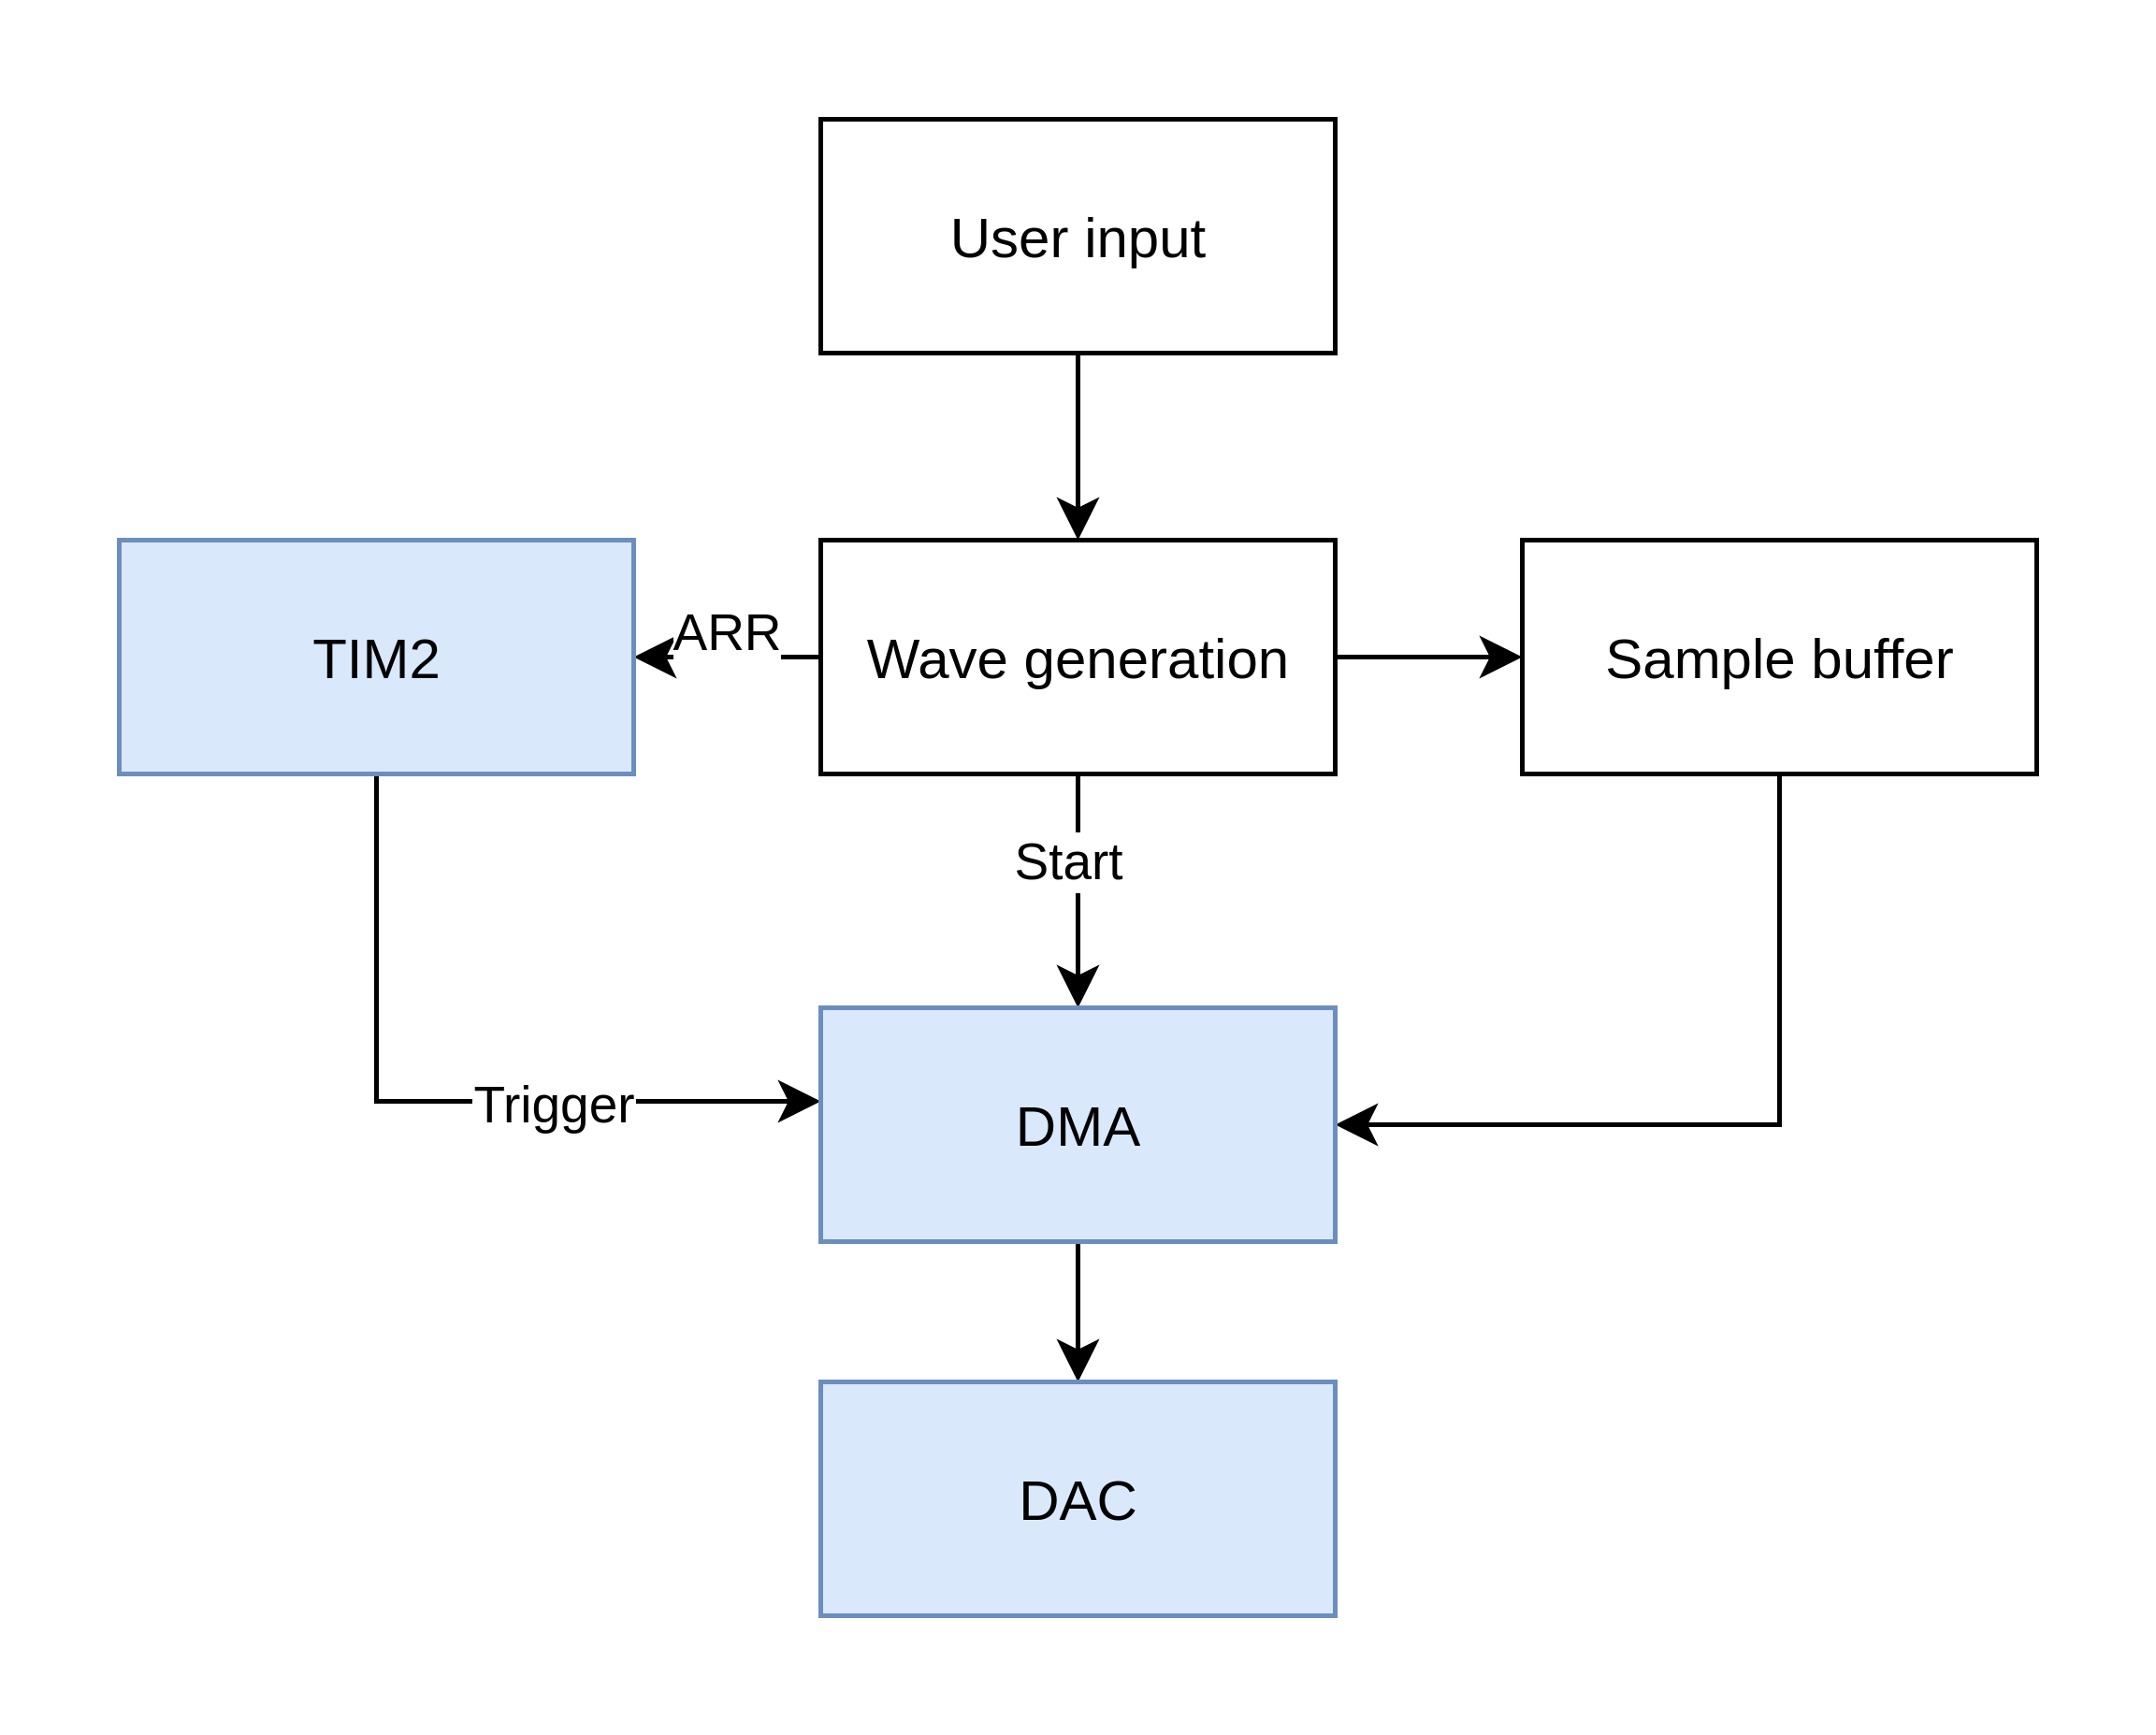
\includegraphics[width=\textwidth]{overview}
      \caption{Design of input capture timer}
      \label{fig:overview}
    \end{figure}

    Figure \ref{fig:overview} shows the basic control flow of the project.
    The important thing to note here is that $1001$ measurements are taken
    because the first tick needs to compare its counter to the event before.
    This is what the reference measurement does.\\

    A UART interface was designed to utilize \code{printf}/\code{getline}
    features to the UART. Input and output via the uart was stardardized to
    more closely resemble a common C program. 

    \section*{Test plan}

    The POST routine was used to test the existence of a wave. To test the actual timer,
    various frequencies were tested to see if the buckets filled around the generated
    frequency. The sum of all buckets was verified to equal $1000$.\\

    To test the UART portion, the limits of the input were tested as well as invalid
    inputs. The \code{DEL} ASCII code was tested to be handled properly during getline
    to allow the user to use backspace during inputs.

    \section*{Project Results}

    When running the program with a \SI{1}{\kilo\Hz} wave connected, I'd expect the
    output to be grouped around \SI{1000}{ms}.
    
    \begin{figure}[h!]
    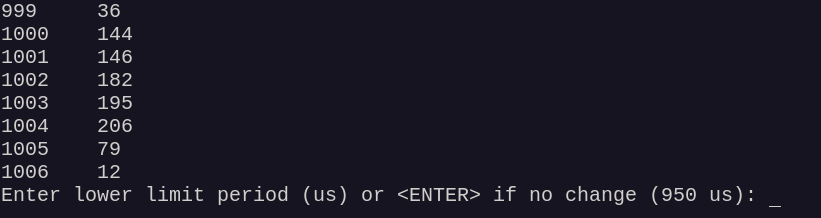
\includegraphics[width=\textwidth]{s1}
    \caption{Input capture performed with a \SI{1}{\kilo\Hz} signal}
    \end{figure}

    When run again with a \SI{2}{\kilo\Hz}, I'd expect the period to be around
    \SI{500}{ms}.

    \begin{figure}[h!]
    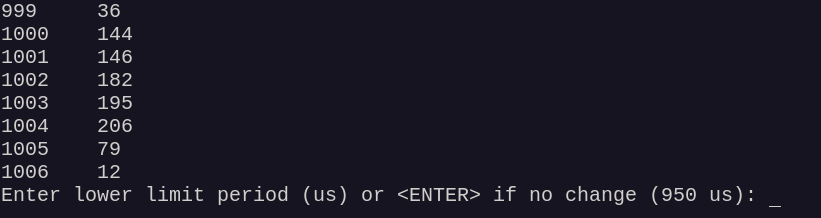
\includegraphics[width=\textwidth]{s1}
    \caption{Input capture performed with a \SI{1}{\kilo\Hz} signal}
    \end{figure}

    Both of the tests run and output expected results.

    \section*{Lessons learned}
    I encountered two major issues while working on the project. The first issue was
    that the wave generator I was using initially was not configured to pulse to the
    correct voltage. The timer would never trip even though the wave looked correct on
    the oscilliscope. The second issue was due to my misunderstanding with how the
    timer works. I assumed that when an input event was triggered, the counter would
    be reset. Due to this assumption, the results would become very skewed after
    re-running the program a couple of times. Once I realized how the timer works
    and the reference measurement was implemented, the program worked properly.

\end{document}
